\documentclass[11pt]{article}

% ============================================================
% Milestone 1 -- Project Proposal & Literature Review Template
% DIP Team Project
% ============================================================
\usepackage[margin=1in]{geometry}
\usepackage[T1]{fontenc}
\usepackage[utf8]{inputenc}
\usepackage{amsmath,amssymb}
\usepackage{graphicx}
\usepackage{booktabs}
\usepackage{array}
\usepackage{tabularx}
\usepackage{float}
\usepackage{ragged2e}
\usepackage[round]{natbib}
\usepackage{hyperref}
\hypersetup{colorlinks=true, linkcolor=blue!50!black, citecolor=blue!50!black, urlcolor=blue!50!black}
\usepackage{enumitem}
\usepackage{xcolor}

\newcommand{\todo}[1]{\textcolor{red}{\textbf{[TODO: #1]}}}
\newcolumntype{Y}{>{\RaggedRight\arraybackslash}X}

\title{\LARGE Project Proposal \& Literature Review \\[4pt]
\large {A9: Remote-Sensing Image Compression for Edge Devices}}
\author{
  \begin{tabular}{ccc}
    Mohamed Ahmed & Ahmed Eid & Randa Medhat \\
    2501902 & 2501923 & 2400036
  \end{tabular}
}
\date{Milestone 1 --- {2/11/2026} \\{} [CSE681] --- Digital Image Processing}

\begin{document}
\sloppy
\maketitle

\begin{center}
\small\textbf{Project repository: }
\url{https://github.com/A7med3id10/LIC-RS-images}
\end{center}

\begin{abstract}
{
Transmitting high-resolution remote-sensing imagery over bandwidth-constrained 
satellite downlinks is a major bottleneck for real-time edge processing. 
This project investigates low-bitrate image compression for aerial imagery 
using a lightweight learned codec suitable for resource-constrained hardware. 
We use the public UC Merced Land Use dataset and reproduce JPEG2000 as the classical baseline. 
We then evaluate a lightweight MeanScale Hyperprior model from the CompressAI framework, 
aiming to minimize bits-per-pixel (bpp) while preserving fidelity in MS-SSIM and PSNR. 
The result will be a reproducible rate-distortion benchmark 
comparing learned and classical compression. 
}
\end{abstract}




\section{Problem Statement \& Motivation}
\label{sec:motivation}
{
Remote-sensing platforms such as CubeSats and UAVs generate large volumes of high-resolution imagery; 
tight power budgets, onboard storage, and narrow bandwidth limit the downlink. 
We address the problem of compressing remote-sensing images at low bitrates 
while keeping the codec lightweight enough for resource-constrained hardware. 
Classical codecs struggle in this system: 
JPEG produces blocking artifacts at very low bitrates, 
and JPEG2000 achieves better quality but at a higher computational cost than JPEG. 
Learned image compression offers better rate-distortion performance, 
so we study whether a lightweight learned codec can outperform JPEG2000 at low bitrates on the UC Merced dataset. 
The project connects directly to the course topics Image Compression ([GW] Ch.8) and Wavelets ([GW] Ch.7): 
JPEG2000 relies on the Discrete Wavelet Transform for energy compaction; 
it then applies quantization to regulate the bitrate 
and entropy coding to compress the resulting coefficients, with rate-distortion theory governing the bpp-fidelity trade-off. 
The learned codec follows the same transform-coding framework but replaces the fixed DWT with a trained neural network encoder.
}



\section{Related Work}
\label{sec:related}

\begin{table}[H]
\centering
\small
\setlength{\tabcolsep}{4pt}
\caption{Key references.}
\label{tab:refs}
\resizebox{\textwidth}{!}{%
\begin{tabular}{@{}p{0.27\linewidth}p{0.12\linewidth}p{0.57\linewidth}@{}}
\toprule
\textbf{Reference} & \textbf{Year} & \textbf{Relevance to this project} \\
\midrule
\citep{wang2025towards} & 2025 & Proposes VMIC, a state-of-the-art remote sensing codec using Mamba, which serves as our primary inspiration. \\
\citep{minnen2018joint} & 2018 & Introduces the Mean-Scale Hyperprior (\texttt{mbt2018\_mean}), the lightweight baseline we adopt for our Edge-focused modifications. \\
\citep{begaint2020compressai} & 2020 & Provides the CompressAI framework used to implement and evaluate our learned codec. \\
\citep{ye2025map} & 2025 & Investigates map-assisted remote-sensing image compression at very low bitrates. \\
\bottomrule
\end{tabular}%
}
\end{table}

Recent research in remote-sensing image compression has explored advanced neural architectures to improve rate--distortion performance. 
Wang et al. propose VMIC, a learned compression network based on the Visual State Space Model (Mamba) \citep{wang2025towards}. 
Mamba introduces a 2D-bidirectional selective scan mechanism, enabling a global effective receptive field with linear computational complexity, which significantly benefits remote-sensing imagery. 
However, the sequential nature of state-space scanning and the heavy channel/global-context entropy modeling introduce computational and memory overheads that are challenging for resource-constrained edge devices, such as satellites. 
To address the constraints of edge deployment, we focus on a more lightweight foundation. 
Minnen et al. introduced the Mean-Scale Hyperprior \citep{minnen2018joint}. 
While their full model (\texttt{mbt2018}) utilizes a slow, autoregressive spatial context model, 
its variant \texttt{mbt2018\_mean} removes this sequential dependency. 
By relying solely on a hierarchical hyperprior to predict both the mean and scale 
of the latent distribution, \texttt{mbt2018\_mean} achieves a strong rate--distortion trade-off 
with significantly faster decoding. 
We adopt this model via the open-source CompressAI framework \citep{begaint2020compressai} as our baseline, 
intending to modify its architecture for edge efficiency. 
Other domain-specific approaches, such as map-assisted compression proposed by Ye et al., target extremely low bitrates by leveraging external information \citep{ye2025map}. 
Unlike these methods, our current work establishes a rigorous benchmark of a lightweight learned codec against JPEG2000 on the UC Merced dataset. 
In future stages, we will modify the \texttt{mbt2018\_mean} baseline by replacing its standard convolutional layers in the encoder and decoder with Depthwise Separable Convolutions to reduce the parameter count and MACs. Additionally, we will integrate a lightweight channel-wise context model inspired by VMIC into its entropy module. This dual approach aims to balance superior compression efficiency with the strict computational limits of edge hardware, avoiding the heavy spatial autoregressive bottleneck.


%------------------------------------------------------------------
\section{Dataset and Data Pipeline}
\label{sec:data}
\subsection{UC Merced Land Use}
We use the UC Merced Land Use dataset: 2{,}100 RGB aerial images of $256\times256$ pixels (about 317~MB), organised in 21 land-use classes with 100 images per class. The folder layout expected by the pipeline is \texttt{root/<class>/<image>.tif}.
 
\subsection{Sanity Check}
Before splitting, every file is opened and fully decoded to detect corrupt files (the script aborts on the first corrupt file). It also counts images whose size differs from $256\times256$ or whose mode is not RGB, so that these can be normalised to the expected format. 
%Number of such images found: \tbd.

\subsection{Seeded, Class-Stratified Split}
For each class independently, file names are sorted, shuffled with a fixed seed (\texttt{random.Random(42)}), and divided into 10\% test, 10\% validation and the remaining 80\% training. With 100 images per class this gives 10/10/80 images per class:
 
\begin{table}[h]
\centering
\caption{Split sizes (seed 42). The split files \texttt{train.csv}, \texttt{val.csv}, \texttt{test.csv} and \texttt{split\_info.json} are committed to the repository so Students~B and~C use identical data.}
\begin{tabular}{lrr}
\toprule
Split & Images per class & Total images \\
\midrule
Train & 80 & 1680 \\
Validation & 10 & 210 \\
Test & 10 & 210 \\
\bottomrule
\end{tabular}
\end{table}
 
All baseline numbers are computed on the \textbf{test} split only.
 
%------------------------------------------------------------------
\subsection{Metric Definitions}

These definitions are fixed for all three students.
 
\paragraph{Bits per pixel.} Computed from the real compressed file size, headers included:
\begin{equation}
  \mathrm{bpp} = \frac{8 \cdot \text{compressed\_bytes}}{H \cdot W}.
\end{equation}
 
\paragraph{PSNR.} On 8-bit RGB, per image, then averaged over the test set:
\begin{equation}
  \mathrm{PSNR} = 10\log_{10}\frac{255^2}{\mathrm{MSE}}.
\end{equation}
 
\paragraph{MS-SSIM.} Computed per image with \texttt{pytorch\_msssim} (\texttt{data\_range}=255, 5 scales, $11\times11$ window).
 
\paragraph{MS-SSIM (dB).} Per image, then averaged, using the same transform as the VMIC paper:
\begin{equation}
  \mathrm{MS\text{-}SSIM_{dB}} = -10\log_{10}\bigl(1-\mathrm{MS\text{-}SSIM}\bigr).
\end{equation}
 
%------------------------------------------------------------------
\subsection{JPEG2000 Baseline Protocol}
%------------------------------------------------------------------
Each test image is encoded and decoded with JPEG2000 using OpenJPEG through Pillow (official wheels include OpenJPEG). Target rates (bpp) are
\[
  \{0.25,\ 0.5,\ 0.75,\ 1.0,\ 1.5,\ 2.0\}.
\]
Because the codec only approximates a target rate, the \emph{actual} bpp is measured from the encoded byte count and reported alongside the quality metrics. A target bpp is converted to a compression ratio relative to 24~bpp RGB (ratio $=24/\text{bpp}$) and passed to OpenJPEG through Pillow with the following settings:
\begin{itemize}
  \item \texttt{quality\_mode="rates"}, \texttt{quality\_layers=[24/bpp]};
  \item \texttt{irreversible=True} (lossy 9/7 wavelet);
  \item \texttt{mct=1} (RGB$\to$YCC colour transform);
  \item \texttt{num\_resolutions=6}.
\end{itemize}
Each image is encoded at every target rate, decoded from the in-memory codestream, and compared to the original. Metrics are computed per image and then averaged over the test set. Per-image and per-class results are also saved (\texttt{jp2k\_per\_image.csv}, \texttt{jp2k\_per\_class.csv}) for Milestone~3.


\subsection{Baseline Results}
%------------------------------------------------------------------
Table~\ref{tab:jp2k} gives the JPEG2000 reference numbers on the 210-image test split (mean over images).
 
\begin{table}[h]
\centering
\caption{JPEG2000 baseline on the UC Merced test split (mean over 210 images).}
\label{tab:jp2k}
\begin{tabular}{@{}ccccc@{}}
\toprule
Target bpp & Actual bpp & PSNR (dB) & MS-SSIM & MS-SSIM (dB) \\
\midrule
0.25 & 0.246 & 27.52 & 0.9255 & 11.65 \\
0.50 & 0.493 & 30.48 & 0.9615 & 14.64 \\
0.75 & 0.744 & 32.45 & 0.9752 & 16.65 \\
1.00 & 0.992 & 33.97 & 0.9820 & 18.14 \\
1.50 & 1.490 & 36.44 & 0.9894 & 20.58 \\
2.00 & 1.989 & 38.50 & 0.9931 & 22.56 \\
\bottomrule
\end{tabular}
\end{table}
 
% Uncomment once the RD plot exists (results/rd_jp2k.png):
% \begin{figure}[h]
%   \centering
%   \includegraphics[width=0.8\linewidth]{results/rd_jp2k.png}
%   \caption{Rate--distortion curve of JPEG2000 (PSNR vs.\ actual bpp).}
% \end{figure}
 

\subsection{Data License}
The Kaggle-hosted copy identifies its license as CC0 1.0 Public Domain
\citep{ucmercedkaggle}. This is the license declared for that mirror; because
the mirror's declaration does not by itself establish the rights to every
upstream image, we will use the data for this research project and will not
redistribute the image files.


\section{Proposed Method}
\label{sec:method}
Our proposed approach builds upon the \texttt{mbt2018\_mean} architecture from CompressAI, 
which uses a Mean-Scale Hyperprior to estimate the entropy of the latent representation. 
This model is a strong baseline: it does not include any spatial autoregressive context, 
making it significantly faster than the full \texttt{mbt2018} model 
while still achieving competitive rate-distortion performance. 
However, our measurement of the default CompressAI configuration (quality level 5) indicates approximately 17.5 million parameters 
which is not optimized for the strict power and memory constraints of edge devices.

Figure~\ref{fig:mean-scale-hyperprior} summarizes the baseline codec's analysis, entropy-coding, and synthesis paths. Given an input image $x$, the analysis transform $g_a$ (the encoder) produces a latent representation $y=g_a(x)$. This representation carries most of the image information, but its values are not equally likely. The codec therefore quantizes $y$ to obtain $\hat{y}$ and entropy-codes it into the main bitstream. At the receiver, arithmetic decoding recovers $\hat{y}$, and the synthesis transform $g_s$ (the decoder) maps it to the reconstructed image $\hat{x}=g_s(\hat{y})$. Quantization makes the representation discrete; entropy coding then assigns shorter codes to more probable values, reducing the number of transmitted bits.

\begin{figure}[htbp]
    \centering
    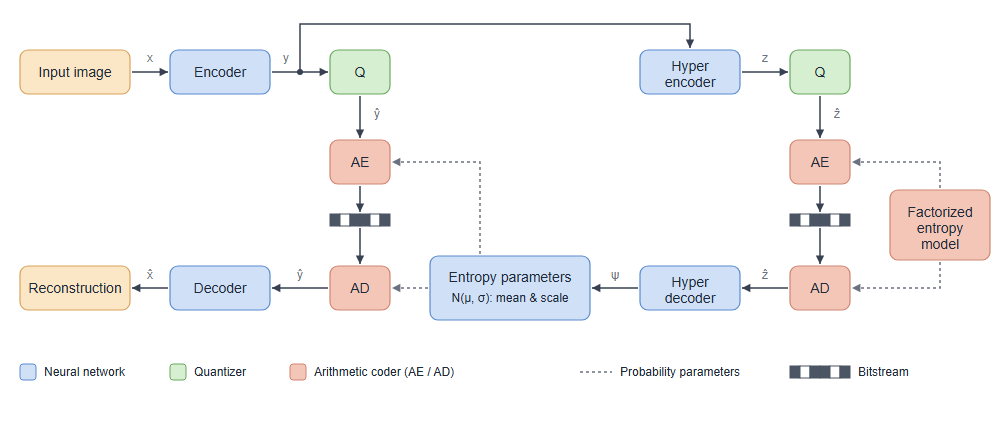
\includegraphics[width=\textwidth]{mean-scale-hyperprior.png}
    \caption{Mean--scale hyperprior autoencoder block diagram.}
    \label{fig:mean-scale-hyperprior}
\end{figure}
The hyperprior sends a second, compact bitstream that helps both encoder and decoder estimate the probability distribution of the main latent representation.
A hyper-analysis transform $h_a$ processes the unquantized latent $y$ to produce a smaller auxiliary representation $z=h_a(y)$. 

The codec quantizes $z$ to $\hat{z}$ and encodes it separately using a factorized entropy model, giving the hyperprior bitstream. At the receiver, this stream is decoded first; a hyper-synthesis transform $h_s$ maps $\hat{z}$ to entropy parameters $\psi=(\mu,\sigma)$ for the main latent. Here, $\mu$ is the predicted mean and $\sigma$ is the predicted scale (standard deviation). Together they define a Gaussian model, conventionally written $\mathcal{N}(\mu,\sigma^2)$, for the latent values. The encoder and decoder use the same predicted parameters when coding and decoding $\hat{y}$. In the diagram, AE and AD denote arithmetic encoding and arithmetic decoding, respectively, and the dotted arrows show where the predicted probability parameters are used.

This two-stream design provides a net benefit: although transmitting the hyperprior $z$ adds a small bitrate cost, it allows the codec to accurately predict the probability distribution of $y$ for the specific input image. This accurate prediction reduces the size of the main bitstream far more than the cost of the side information. Notably, the \texttt{mbt2018\_mean} baseline relies solely on this hyperprior for probability estimation, avoiding any sequential spatial context (unlike the full \texttt{mbt2018} model), which enables fast, parallel decoding.

The figure describes our baseline. Our contribution is twofold, aiming to reduce computation while improving probability estimates:

\begin{enumerate}
    \item \textbf{Lightweight Architecture:} We will replace the standard $5\times5$ convolutional layers in the encoder ($g_a$) and decoder ($g_s$) with Depthwise Separable Convolutions. This reduces the number of parameters and Multiply-Accumulate operations (MACs) while maintaining representational capacity.
    \item \textbf{Efficient Entropy Modeling with Channel-wise Context:} Since \texttt{mbt2018\_mean} lacks any form of context modeling, we will integrate a lightweight Channel-wise Context module into its entropy model. Instead of relying on a slow spatial autoregressive context, we will split the latent representation into channel slices and use inexpensive convolutions to predict the parameters of the current slice based on previously decoded slices. This improves compression efficiency without introducing a sequential decoding bottleneck.
\end{enumerate}

We expect this modified architecture to maintain competitive rate-distortion performance compared to JPEG2000, while offering a significantly lower computational footprint suitable for edge deployment.

\section{Feasibility \& Compute Plan}
\label{sec:feasibility}

The project is CPU-OK and its minimum viable comparison requires no model
training: we evaluate CompressAI's pretrained \texttt{mbt2018\_mean} at quality
levels 1--8 against JPEG2000. We have already run this pipeline on a pilot
subset of 20 UC Merced images selected with random seed 42. This 20-image
comparison is the MVP; expanding the evaluation to 100 images from the same
seeded selection is the next step if it fits the compute budget. We budget up
to one working day for the 100-image evaluation on an 8-core CPU with 16 GB
RAM; an optional entry-level GPU may shorten this time but is not required.
The MVP uses pretrained weights, so it requires no custom-model training.

Figure~\ref{fig:preliminary-rd} presents the completed pilot comparison. For
each of the 20 images, the evaluation script measures the pretrained model at
quality levels 1--8 and encodes JPEG2000 at a target rate based on the learned
codec's bitrate; the plotted bitrate and PSNR values are averages over the
images. The learned model's curve is higher at the plotted operating points
on this pilot subset. This is encouraging evidence that the pipeline runs and
provides a useful initial comparison, but it does not establish that the same
gap holds across the planned 100-image evaluation. The plot reports the
pretrained baseline, not our proposed lightweight modifications.

\begin{figure}[H]
    \centering
    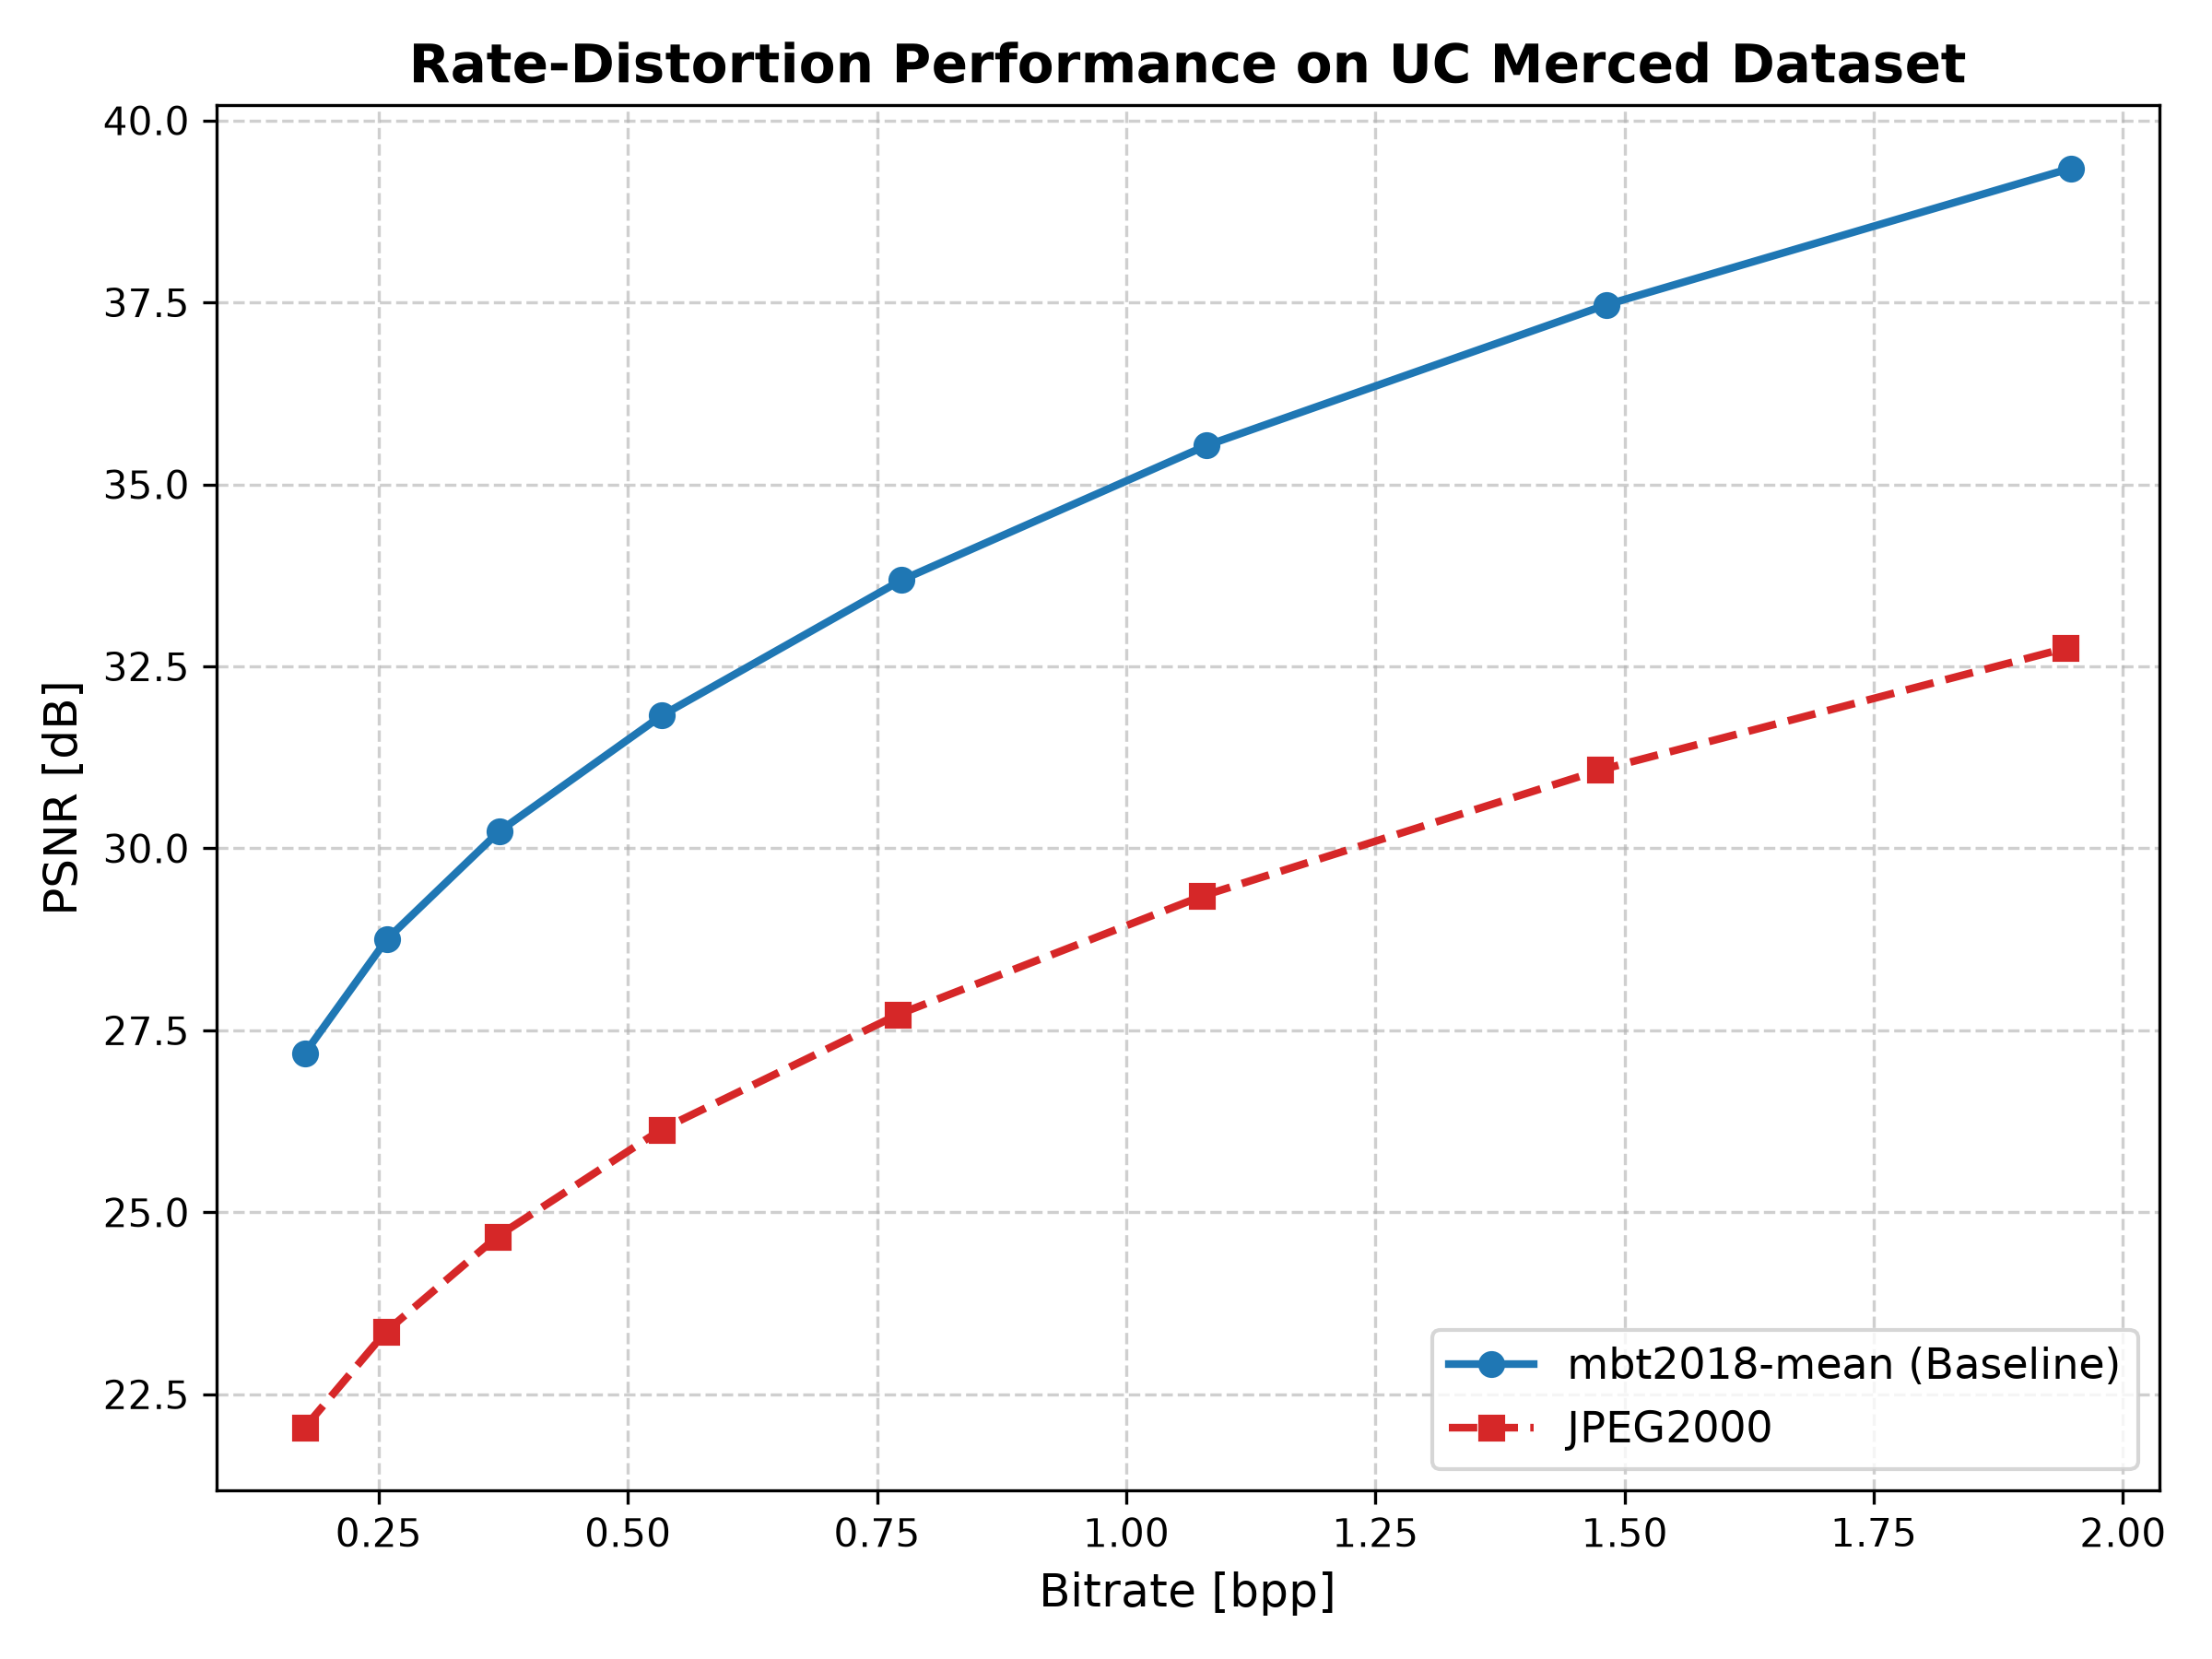
\includegraphics[width=0.58\textwidth]{rd_curve.png}
    \caption{Pilot rate--distortion curves for pretrained \texttt{mbt2018\_mean} and JPEG2000 (20 UC Merced images).}
    \label{fig:preliminary-rd}
\end{figure}

\subsection{Minimum Viable Deliverable (MVP)}
A reproducible rate--distortion comparison of pretrained
\texttt{mbt2018\_mean} and JPEG2000 on the same UC Merced image subset. We will
report actual bits per pixel (bpp) and PSNR for each codec, along with the
image count, selection seed, software versions, and measured runtime. The
20-image pilot has been run and supplies the current MVP comparison; we will
document its per-quality measurements and runtime, then extend the same
protocol to 100 images if it fits the compute budget.

\subsection{Stretch Goal}
If the MVP is on track by Week 5--6, we will implement and evaluate our primary contribution: the proposed lightweight codec modifications (Depthwise Separable Convolutions and Channel-wise Context). We will compare this modified model against both the pretrained baseline and JPEG2000. Crucially, we will measure the rate-distortion performance alongside practical edge-metrics such as encoding/decoding time and peak memory use. 

While this lightweight extension represents the core objective of our project, we adopt a risk-mitigated approach: should the training or 100-image expansion exceed our compute budget, the project will still be considered complete and reportable based on the rigorous MVP baseline comparison.



\section{Risk Assessment}
\label{sec:risk}
\begin{itemize}[leftmargin=*]
  \item \textbf{Risk 1:} The pretrained \texttt{mbt2018\_mean} model was trained on natural images and may not generalize to remote-sensing imagery. \textbf{Mitigation:} The completed 20-image pilot provides an initial comparison, not a dataset-wide conclusion. We will report the results on the fixed pilot sample honestly and, if the budget allows, repeat the same protocol on 100 images before drawing broader conclusions. Fine-tuning on UC Merced is an optional extension, not a requirement for the MVP.
  \item \textbf{Risk 2:} The 100-image evaluation or lightweight model extension may exceed the laptop-class compute budget, or the modifications may reduce rate--distortion performance. \textbf{Mitigation:} The MVP is the completed 20-image pretrained-baseline comparison and needs no custom training. We will prioritize reporting its bpp, PSNR, sample size, seed, and runtime; the 100-image expansion and proposed model changes are subsequent work. If the extension is infeasible or performs poorly, we will retain the pretrained baseline as the primary result and report the modified model's measured complexity and performance without overstating improvements.
\end{itemize}



\section{Work Breakdown}
\label{sec:workbreakdown}
\begin{table}[H]
\centering
\small
\caption{Milestone task allocation and deliverables.}
\label{tab:tasks}
\begin{tabularx}{\textwidth}{@{}>{\centering\arraybackslash}p{0.06\textwidth}>{\centering\arraybackslash}p{0.07\textwidth}Y Y Y >{\RaggedRight\arraybackslash}p{0.24\textwidth}@{}}
\toprule
\textbf{M} & \textbf{Wk} &
\textbf{Mohamed Ahmed\newline Data \& Baseline} &
\textbf{Ahmed Eid\newline Model\newline Algorithm} &
\textbf{Randa Medhat\newline Evaluation} &
\textbf{Deliverable} \\
\midrule
1 & 3 &
UC Merced pipeline; JPEG2000 reference numbers &
Scope lightweight codec architecture for remote-sensing statistics &
Define rate--distortion comparison protocol &
Proposal and JPEG2000 baseline table \\
2 & 6 &
Full JPEG2000 rate--distortion curve &
Train small codec; produce first checkpoint &
Preliminary rate--distortion curve versus JPEG2000 &
Progress report and rate--distortion plot \\
3 & 9 &
Final JPEG2000 numbers across classes &
Final codec and per-land-use-class breakdown &
Full rate--distortion comparison and qualitative crops &
Final report, repository, and demo \\
\bottomrule
\end{tabularx}
\end{table}




\clearpage
\bibliographystyle{unsrtnat}
\bibliography{references}

\end{document}